\chapter{Optical Medical Imaging}
\label{ch:optical_imaging}

% Chapter-opening illustrated modality infographic.
\begin{center}
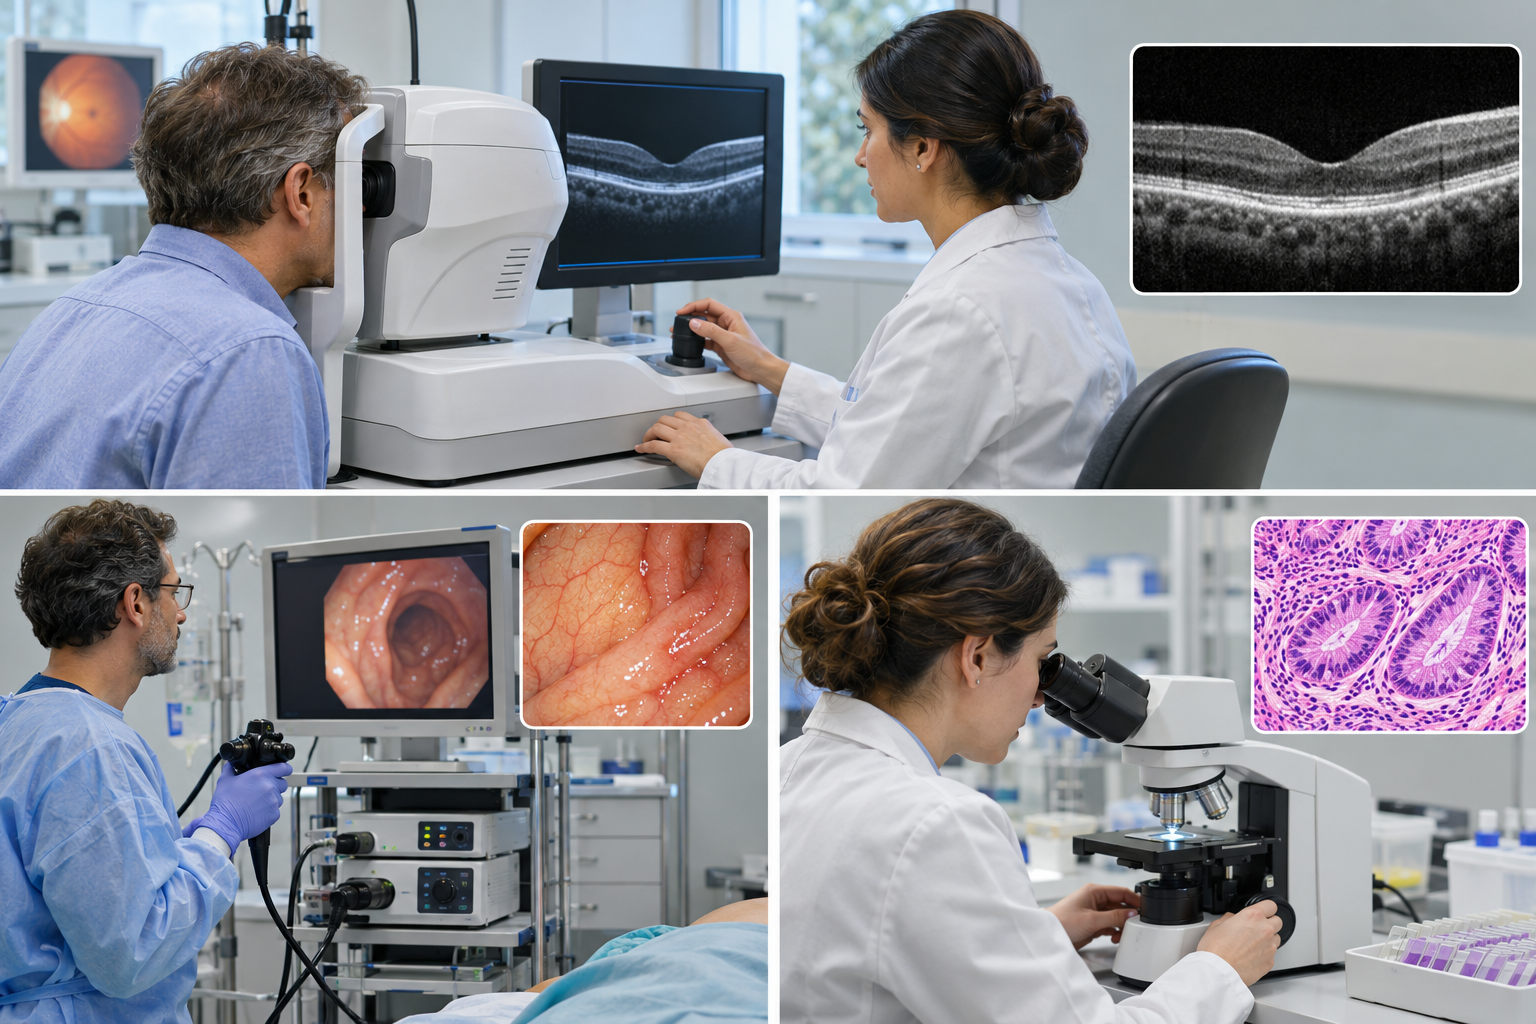
\includegraphics[width=\textwidth,keepaspectratio]{modalities/infographics/optical_realistic.png}
\end{center}
\begin{center}\footnotesize Optical methods include OCT, endoscopy, and microscopy; they reveal structure at different scales, while tissue scattering limits depth. AI-generated illustration; all image panels are illustrative.\end{center}

\section{Overview}
Optical imaging encompasses medical imaging techniques that use ultraviolet, visible, near-infrared, or infrared light to visualize anatomical structures, tissue microarchitecture, vascular networks, cellular morphology, biochemical composition, and physiological activity.

Unlike X-ray, CT, and nuclear medicine, optical imaging does not use ionizing radiation. Its principal limitation is the absorption and scattering of light within biological tissues, which restricts imaging penetration depth. Optical imaging can provide exceptionally high spatial resolution, from macroscopic anatomical visualization to subcellular characterization.

\begin{center}
\begin{tabular}{@{}p{0.32\textwidth}p{0.31\textwidth}p{0.29\textwidth}@{}}
\toprule
\textbf{Imaging modality} & \textbf{Physical principle} & \textbf{Primary clinical application} \\
\midrule
Autofluorescence imaging & Endogenous tissue fluorescence & Retinal and epithelial abnormalities \\
Confocal microscopy & Spatially filtered optical detection & Cellular and tissue microstructure \\
Conventional medical photography & Visible light reflection & Dermatology, wound assessment \\
Dermoscopy & Magnified polarized or nonpolarized light & Skin lesion characterization \\
Diffuse optical tomography (DOT) & Diffuse photon propagation & Functional tissue imaging \\
Digital optical microscopy & Magnified transmitted or reflected light & Histopathology and cytopathology \\
Endoscopy & Direct optical visualization & Gastrointestinal and respiratory diseases \\
Fluorescence angiography & Fluorescent dye excitation and emission & Retinal and vascular imaging \\
Fluorescence imaging & Endogenous or exogenous fluorescence & Tumor and tissue visualization \\
Fluorescence lifetime imaging & Fluorescence decay characteristics & Tissue metabolic characterization \\
Functional NIRS (fNIRS) & Hemodynamic optical signal variation & Functional brain imaging \\
Fundus photography & Retinal light reflection & Retinal diseases \\
Hyperspectral imaging & Wavelength-dependent tissue reflectance & Tissue oxygenation and characterization \\
Infrared thermography & Naturally emitted infrared radiation & Surface temperature distribution \\
Laser speckle contrast imaging & Speckle variation caused by blood flow & Microcirculatory assessment \\
Multiphoton microscopy & Nonlinear optical excitation & Cellular and extracellular structure \\
Narrow-band imaging (NBI) & Wavelength-selective illumination & Epithelial and vascular abnormalities \\
Near-infrared spectroscopy (NIRS) & Wavelength-dependent optical absorption & Tissue oxygenation \\
OCT angiography (OCTA) & Motion-dependent optical signal variation & Retinal microvascular imaging \\
Optical coherence tomography (OCT) & Low-coherence interferometry & Ophthalmology, cardiology \\
Photoacoustic imaging & Optical absorption and acoustic detection & Vascular and functional imaging \\
Raman spectroscopy and imaging & Inelastic photon scattering & Molecular tissue characterization \\
Reflectance confocal microscopy & Backscattered light & Dermatological imaging \\
Second-harmonic generation imaging & Nonlinear frequency conversion & Collagen and fibrous tissue \\
\bottomrule
\end{tabular}
\end{center}

Optical imaging should be treated as a family of distinct modalities, rather than as a single technique. The catalogue includes ophthalmic imaging, endoscopy, dermatology, digital pathology, and other optical methods. Some findings are nonspecific, and several applications remain investigational.

\section{Where optical imaging is used}
The following numbered entries present examples of optical findings and techniques. Optical appearance depends on illumination, wavelength, acquisition geometry, instrument settings, and tissue properties; many findings require clinical or histopathological correlation.

\subsection{Retinal diseases}
\begin{enumerate}[leftmargin=*,itemsep=0.45em,topsep=0.4em]
\item \textbf{Best vitelliform macular dystrophy.} Useful imaging findings include: OCT, autofluorescence. Characteristic Imaging Findings: Vitelliform subretinal deposits.
\item \textbf{Branch retinal artery occlusion.} Useful imaging findings include: OCT, fundus photography. Characteristic Imaging Findings: Sectoral retinal ischemic abnormalities.
\item \textbf{Central retinal artery occlusion.} Useful imaging findings include: Fundus photography, OCT. Characteristic Imaging Findings: Retinal whitening and acute inner retinal hyperreflectivity.
\item \textbf{Central serous chorioretinopathy.} Useful imaging findings include: OCT. Characteristic Imaging Findings: Serous neurosensory retinal detachment.
\item \textbf{Choroidal neovascularization.} Useful imaging findings include: OCTA, fluorescein angiography. Characteristic Imaging Findings: Abnormal vascular network beneath or within the retina.
\item \textbf{Coats disease.} Coats disease is an abnormal retinal telangiectasia with leakage; imaging assesses exudation and retinal detachment. Useful imaging findings include: Fundus photography, angiography. Characteristic Imaging Findings: Retinal telangiectasia and exudation.
\item \textbf{Diabetic macular edema.} Useful imaging findings include: OCT. Characteristic Imaging Findings: Retinal thickening and intraretinal cystic spaces.
\item \textbf{Diabetic retinopathy.} Useful imaging findings include: Fundus photography. Characteristic Imaging Findings: Microaneurysms, hemorrhages, hard exudates.
\item \textbf{Dry age-related macular degeneration.} Useful imaging findings include: OCT, fundus photography. Characteristic Imaging Findings: Drusen and retinal pigment epithelial abnormalities.
\item \textbf{Epiretinal membrane.} Useful imaging findings include: OCT. Characteristic Imaging Findings: Hyperreflective membrane along retinal surface.
\item \textbf{Geographic atrophy.} Geographic atrophy is progressive loss of retinal pigment epithelium and outer retina in age-related macular degeneration; imaging maps its extent. Useful imaging findings include: Fundus autofluorescence, OCT. Characteristic Imaging Findings: Reduced autofluorescence and outer retinal atrophy.
\item \textbf{Hydroxychloroquine retinopathy.} Useful imaging findings include: OCT, autofluorescence. Characteristic Imaging Findings: Parafoveal or pericentral outer retinal degeneration.
\item \textbf{Hypertensive retinopathy.} Useful imaging findings include: Fundus photography. Characteristic Imaging Findings: Arteriolar narrowing, hemorrhages and cotton-wool spots.
\item \textbf{Macular hole.} Useful imaging findings include: OCT. Characteristic Imaging Findings: Full-thickness or partial-thickness foveal defect.
\item \textbf{Neovascular age-related macular degeneration.} Useful imaging findings include: OCT, OCTA. Characteristic Imaging Findings: Neovascular complexes, subretinal or intraretinal fluid.
\item \textbf{Proliferative diabetic retinopathy.} Useful imaging findings include: Fundus photography, fluorescein angiography. Characteristic Imaging Findings: Retinal neovascularization and vascular leakage.
\item \textbf{Retinal detachment.} Useful imaging findings include: Fundus photography, OCT. Characteristic Imaging Findings: Separation of neurosensory retina from underlying tissue; OCT assesses scanned regions, while peripheral extent requires a dilated retinal examination.
\item \textbf{Retinal tear.} Useful imaging findings include: Wide-field fundus imaging. Characteristic Imaging Findings: Discontinuity in peripheral retinal tissue.
\item \textbf{Retinal telangiectasia.} Useful imaging findings include: OCTA, fluorescein angiography. Characteristic Imaging Findings: Abnormal dilated retinal capillaries.
\item \textbf{Retinal vasculitis.} Useful imaging findings include: Fluorescein angiography. Characteristic Imaging Findings: Vascular staining and leakage.
\item \textbf{Retinal vein occlusion.} Useful imaging findings include: Fundus photography, fluorescein angiography. Characteristic Imaging Findings: Retinal hemorrhages, venous dilatation and delayed drainage.
\item \textbf{Retinitis pigmentosa.} Useful imaging findings include: OCT, fundus autofluorescence. Characteristic Imaging Findings: Outer retinal degeneration and characteristic autofluorescent abnormalities.
\item \textbf{Retinopathy of prematurity.} Useful imaging findings include: Wide-field retinal imaging. Characteristic Imaging Findings: Abnormal peripheral retinal vascular development.
\item \textbf{Stargardt disease.} Stargardt disease is an inherited macular dystrophy associated with lipofuscin accumulation; imaging assesses characteristic deposits and atrophy. Useful imaging findings include: Fundus autofluorescence, OCT. Characteristic Imaging Findings: Abnormal lipofuscin distribution and macular atrophy.
\item \textbf{Vitreomacular traction.} Useful imaging findings include: OCT. Characteristic Imaging Findings: Persistent vitreous attachment with foveal distortion.
\item \textbf{Vitreous hemorrhage.} Useful imaging findings include: Fundus photography. Characteristic Imaging Findings: Obscured retinal visualization from intraocular blood.
\end{enumerate}

\subsection{Glaucoma and optic nerve disorders}
\begin{enumerate}[leftmargin=*,itemsep=0.45em,topsep=0.4em]
\item \textbf{Compressive optic neuropathy.} Useful imaging findings include: OCT. Characteristic Imaging Findings: Characteristic patterns of ganglion cell and nerve fiber loss.
\item \textbf{Ischemic optic neuropathy.} Useful imaging findings include: OCT, fundus photography. Characteristic Imaging Findings: Optic disc edema followed by sectoral atrophy.
\item \textbf{Juvenile glaucoma.} Useful imaging findings include: OCT. Characteristic Imaging Findings: Optic nerve head and retinal nerve fiber abnormalities.
\item \textbf{Normal-tension glaucoma.} Useful imaging findings include: OCT. Characteristic Imaging Findings: Retinal nerve fiber and ganglion cell loss.
\item \textbf{Optic atrophy.} Useful imaging findings include: OCT, fundus photography. Characteristic Imaging Findings: Optic disc pallor and nerve fiber loss.
\item \textbf{Optic disc drusen.} Useful imaging findings include: Enhanced-depth OCT. Characteristic Imaging Findings: Characteristic buried or superficial optic nerve head deposits.
\item \textbf{Optic neuritis.} Useful imaging findings include: OCT. Characteristic Imaging Findings: Acute swelling or subsequent retinal nerve fiber thinning.
\item \textbf{Papilledema.} Useful imaging findings include: OCT, fundus photography. Characteristic Imaging Findings: Optic disc swelling and increased nerve fiber thickness.
\item \textbf{Pigmentary glaucoma.} Useful imaging findings include: Slit-lamp imaging, OCT. Characteristic Imaging Findings: Pigment deposition and glaucomatous damage.
\item \textbf{Primary angle-closure glaucoma.} Useful imaging findings include: Anterior segment OCT, optic nerve OCT. Characteristic Imaging Findings: Narrow anterior chamber angle and glaucomatous structural damage.
\item \textbf{Primary open-angle glaucoma.} Useful imaging findings include: OCT. Characteristic Imaging Findings: Retinal nerve fiber layer thinning.
\item \textbf{Pseudoexfoliative glaucoma.} Useful imaging findings include: Slit-lamp imaging, OCT. Characteristic Imaging Findings: Pseudoexfoliative material and optic nerve damage.
\end{enumerate}
Optical imaging can quantify structural glaucomatous damage, but glaucoma diagnosis also requires clinical assessment, intraocular pressure measurements, visual field testing, and, where appropriate, gonioscopy.

\subsection{Corneal and anterior segment disorders}
\begin{enumerate}[leftmargin=*,itemsep=0.45em,topsep=0.4em]
\item \textbf{Acanthamoeba keratitis.} Acanthamoeba keratitis is a corneal infection that can cause severe pain and stromal injury; confocal findings can support, but do not replace, microbiological assessment. Useful imaging findings include: Confocal microscopy. Characteristic Imaging Findings: Characteristic cyst-like structures.
\item \textbf{Anterior uveitis.} Anterior uveitis is inflammation within the anterior eye; slit-lamp examination identifies cells and flare. Useful imaging findings include: Slit-lamp imaging. Characteristic Imaging Findings: Inflammatory cells and flare.
\item \textbf{Bacterial keratitis.} Bacterial keratitis is corneal infection; imaging documents the infiltrate and epithelial defect, while microbiology may guide treatment. Useful imaging findings include: Slit-lamp imaging. Characteristic Imaging Findings: Corneal infiltrate and epithelial defect.
\item \textbf{Cataract.} Useful imaging findings include: Slit-lamp photography, Scheimpflug imaging. Characteristic Imaging Findings: Lens opacity.
\item \textbf{Corneal dystrophy.} Useful imaging findings include: Confocal microscopy, OCT. Characteristic Imaging Findings: Abnormal corneal deposits.
\item \textbf{Corneal edema.} Useful imaging findings include: OCT. Characteristic Imaging Findings: Increased corneal thickness.
\item \textbf{Corneal scarring.} Useful imaging findings include: OCT. Characteristic Imaging Findings: Abnormal stromal reflectivity.
\item \textbf{Corneal ulcer.} Useful imaging findings include: Slit-lamp imaging, OCT. Characteristic Imaging Findings: Epithelial defect and stromal inflammation.
\item \textbf{Dry eye disease.} Dry eye disease reflects tear-film instability or inadequate tear production; optical assessment examines tear-film and ocular-surface changes. Useful imaging findings include: Optical tear film imaging. Characteristic Imaging Findings: Tear film instability and altered tear meniscus.
\item \textbf{Fuchs endothelial dystrophy.} Fuchs endothelial dystrophy is a progressive corneal endothelial disorder; imaging assesses guttata, cell loss, and corneal edema. Useful imaging findings include: Specular microscopy. Characteristic Imaging Findings: Endothelial cell abnormalities and guttata.
\item \textbf{Fungal keratitis.} Fungal keratitis is corneal infection that may involve deeper stromal tissue; confocal findings can help target microbiological sampling. Useful imaging findings include: Confocal microscopy. Characteristic Imaging Findings: Possible filamentous fungal structures.
\item \textbf{Herpes simplex keratitis.} Herpes simplex keratitis is viral corneal infection; fluorescein-assisted examination can show characteristic epithelial lesions. Useful imaging findings include: Fluorescein-assisted slit-lamp imaging. Characteristic Imaging Findings: Dendritic epithelial lesions.
\item \textbf{Hyphema.} Hyphema is blood in the anterior chamber, usually after trauma; imaging documents its extent when direct examination is limited. Useful imaging findings include: Anterior segment photography. Characteristic Imaging Findings: Blood within the anterior chamber.
\item \textbf{Iris melanoma.} Useful imaging findings include: Anterior segment photography, OCT. Characteristic Imaging Findings: Pigmented iris mass with abnormal morphology.
\item \textbf{Keratoconus.} Keratoconus is progressive corneal thinning and irregular steepening; tomography assesses shape and severity. Useful imaging findings include: Corneal tomography, OCT. Characteristic Imaging Findings: Corneal thinning and abnormal curvature.
\item \textbf{Keratoglobus.} Keratoglobus is diffuse corneal thinning with globular protrusion; tomography maps corneal thickness and contour. Useful imaging findings include: Corneal tomography. Characteristic Imaging Findings: Diffuse corneal thinning and protrusion.
\item \textbf{Meibomian gland dysfunction.} Meibomian gland dysfunction impairs the lipid layer of the tear film; infrared meibography can show gland dropout or distortion. Useful imaging findings include: Infrared meibography. Characteristic Imaging Findings: Gland shortening, distortion or dropout.
\item \textbf{Pellucid marginal degeneration.} Useful imaging findings include: Corneal tomography. Characteristic Imaging Findings: Inferior peripheral corneal thinning.
\item \textbf{Posterior capsular opacification.} Useful imaging findings include: Slit-lamp photography. Characteristic Imaging Findings: Opacification of the posterior lens capsule.
\item \textbf{Pterygium.} Pterygium is fibrovascular conjunctival tissue extending onto the cornea; imaging assesses corneal involvement and induced distortion. Useful imaging findings include: Slit-lamp photography, OCT. Characteristic Imaging Findings: Fibrovascular tissue extending onto the cornea.
\end{enumerate}

\subsection{Dermatological malignancies}
\begin{enumerate}[leftmargin=*,itemsep=0.45em,topsep=0.4em]
\item \textbf{Acral melanoma.} Useful imaging findings include: Dermoscopy. Characteristic Imaging Findings: Irregular pigmentation, sometimes parallel ridge pattern.
\item \textbf{Actinic keratosis.} Actinic keratosis is a sun-related keratinocytic lesion with potential for progression; optical examination helps select lesions for biopsy or treatment. Useful imaging findings include: Dermoscopy, confocal microscopy. Characteristic Imaging Findings: Surface keratin and atypical epidermal architecture.
\item \textbf{Amelanotic melanoma.} Useful imaging findings include: Dermoscopy. Characteristic Imaging Findings: Atypical polymorphous vessels.
\item \textbf{Basal cell carcinoma.} Useful imaging findings include: Dermoscopy. Characteristic Imaging Findings: Arborizing vessels, blue-gray structures and ulceration.
\item \textbf{Cutaneous T-cell lymphoma.} Useful imaging findings include: Dermoscopy. Characteristic Imaging Findings: Variable vascular and scaling patterns.
\item \textbf{Dermatofibrosarcoma protuberans.} Useful imaging findings include: Dermoscopy. Characteristic Imaging Findings: Variable pigmentation and vascular abnormalities.
\item \textbf{Extramammary Paget disease.} Useful imaging findings include: Dermoscopy, confocal microscopy. Characteristic Imaging Findings: Atypical intraepidermal cellular structures.
\item \textbf{Lentigo maligna.} Lentigo maligna is melanoma in situ on chronically sun-damaged skin; dermoscopy and confocal microscopy help define suspicious margins. Useful imaging findings include: Dermoscopy, reflectance confocal microscopy. Characteristic Imaging Findings: Irregular follicular pigmentation and atypical melanocytes.
\item \textbf{Malignant melanoma.} Useful imaging findings include: Dermoscopy. Characteristic Imaging Findings: Atypical pigment network and asymmetric structures.
\item \textbf{Merkel cell carcinoma.} Useful imaging findings include: Dermoscopy. Characteristic Imaging Findings: Nonspecific atypical vascular structures.
\item \textbf{Nodular melanoma.} Useful imaging findings include: Dermoscopy. Characteristic Imaging Findings: Atypical vascular and pigmented structures.
\item \textbf{Squamous cell carcinoma.} Useful imaging findings include: Dermoscopy. Characteristic Imaging Findings: Keratin accumulation and abnormal vessels.
\item \textbf{Squamous cell carcinoma in situ.} Useful imaging findings include: Dermoscopy. Characteristic Imaging Findings: Glomerular vessels and scaling.
\item \textbf{Superficial basal cell carcinoma.} Useful imaging findings include: OCT, dermoscopy. Characteristic Imaging Findings: Abnormal superficial epithelial tumor structures.
\end{enumerate}
Histopathological examination remains essential for definitive diagnosis of many cutaneous malignancies.

\subsection{Benign skin lesions}
\begin{enumerate}[leftmargin=*,itemsep=0.45em,topsep=0.4em]
\item \textbf{Angiokeratoma.} Useful imaging findings include: Dermoscopy. Characteristic Imaging Findings: Dark vascular lacunae.
\item \textbf{Blue nevus.} Useful imaging findings include: Dermoscopy. Characteristic Imaging Findings: Homogeneous blue pigmentation.
\item \textbf{Café-au-lait macule.} Useful imaging findings include: Medical photography. Characteristic Imaging Findings: Uniformly pigmented macule.
\item \textbf{Cherry angioma.} Useful imaging findings include: Dermoscopy. Characteristic Imaging Findings: Red vascular lacunae.
\item \textbf{Dermatofibroma.} Useful imaging findings include: Dermoscopy. Characteristic Imaging Findings: Central white scar-like area with peripheral pigmentation.
\item \textbf{Epidermoid cyst.} Useful imaging findings include: Dermoscopy, photography. Characteristic Imaging Findings: Central punctum and superficial structural changes.
\item \textbf{Melanocytic nevus.} Useful imaging findings include: Dermoscopy. Characteristic Imaging Findings: Regular pigment network or globular pattern.
\item \textbf{Milia.} Useful imaging findings include: Dermoscopy. Characteristic Imaging Findings: Small white-yellow keratin-containing structures.
\item \textbf{Molluscum contagiosum.} Useful imaging findings include: Dermoscopy. Characteristic Imaging Findings: Central umbilication and peripheral vessels.
\item \textbf{Pyogenic granuloma.} Useful imaging findings include: Dermoscopy. Characteristic Imaging Findings: Red homogeneous vascular area and possible white collarette.
\item \textbf{Sebaceous hyperplasia.} Useful imaging findings include: Dermoscopy. Characteristic Imaging Findings: Yellow lobules with peripheral vessels.
\item \textbf{Seborrheic keratosis.} Useful imaging findings include: Dermoscopy. Characteristic Imaging Findings: Milia-like cysts and comedo-like openings.
\item \textbf{Solar lentigo.} Useful imaging findings include: Dermoscopy. Characteristic Imaging Findings: Relatively uniform pigmentation.
\item \textbf{Spitz nevus.} Useful imaging findings include: Dermoscopy. Characteristic Imaging Findings: Starburst or other characteristic patterns.
\item \textbf{Viral wart.} Useful imaging findings include: Dermoscopy. Characteristic Imaging Findings: Papillary structures and thrombosed capillaries.
\end{enumerate}

\subsection{Inflammatory and infectious skin diseases}
\begin{enumerate}[leftmargin=*,itemsep=0.45em,topsep=0.4em]
\item \textbf{Acne vulgaris.} Useful imaging findings include: Medical photography. Characteristic Imaging Findings: Comedones, papules, pustules and nodules.
\item \textbf{Atopic dermatitis.} Useful imaging findings include: Dermoscopy. Characteristic Imaging Findings: Patchy vascular structures and yellow scales.
\item \textbf{Bullous pemphigoid.} Useful imaging findings include: Medical photography. Characteristic Imaging Findings: Tense cutaneous blisters.
\item \textbf{Cutaneous candidiasis.} Useful imaging findings include: Medical photography. Characteristic Imaging Findings: Erythema and satellite lesions.
\item \textbf{Demodicosis.} Useful imaging findings include: Dermoscopy. Characteristic Imaging Findings: Follicular protrusions and abnormalities.
\item \textbf{Discoid lupus erythematosus.} Useful imaging findings include: Dermoscopy. Characteristic Imaging Findings: Follicular plugging and pigmentary abnormalities.
\item \textbf{Erythrasma.} Useful imaging findings include: Wood lamp imaging. Characteristic Imaging Findings: Coral-red fluorescence.
\item \textbf{Hidradenitis suppurativa.} Useful imaging findings include: Medical photography. Characteristic Imaging Findings: Nodules, draining tunnels and scarring.
\item \textbf{Lichen planus.} Useful imaging findings include: Dermoscopy. Characteristic Imaging Findings: Wickham striae.
\item \textbf{Melasma.} Useful imaging findings include: Dermoscopy. Characteristic Imaging Findings: Reticulated facial pigmentation.
\item \textbf{Pemphigus vulgaris.} Useful imaging findings include: Medical photography. Characteristic Imaging Findings: Flaccid blisters and erosions.
\item \textbf{Pityriasis versicolor.} Useful imaging findings include: Wood lamp imaging, dermoscopy. Characteristic Imaging Findings: Variable fluorescence and fine scaling.
\item \textbf{Porphyria cutanea tarda.} Useful imaging findings include: Medical photography. Characteristic Imaging Findings: Blistering and skin fragility.
\item \textbf{Psoriasis.} Useful imaging findings include: Dermoscopy. Characteristic Imaging Findings: Regularly distributed dotted vessels and white scales.
\item \textbf{Rosacea.} Useful imaging findings include: Dermoscopy. Characteristic Imaging Findings: Polygonal vascular networks.
\item \textbf{Scabies.} Useful imaging findings include: Dermoscopy. Characteristic Imaging Findings: Mite-associated triangular structure and burrow.
\item \textbf{Seborrheic dermatitis.} Useful imaging findings include: Dermoscopy. Characteristic Imaging Findings: Yellow scaling and irregular vascular patterns.
\item \textbf{Tinea capitis.} Useful imaging findings include: Trichoscopy. Characteristic Imaging Findings: Comma hairs, corkscrew hairs and broken hairs.
\item \textbf{Tinea corporis.} Useful imaging findings include: Dermoscopy. Characteristic Imaging Findings: Peripheral scaling.
\item \textbf{Vitiligo.} Useful imaging findings include: Wood lamp imaging. Characteristic Imaging Findings: Accentuated depigmented regions.
\end{enumerate}

\subsection{Hair and nail disorders}
\begin{enumerate}[leftmargin=*,itemsep=0.45em,topsep=0.4em]
\item \textbf{Alopecia areata.} Useful imaging findings include: Trichoscopy. Characteristic Imaging Findings: Yellow dots, black dots and exclamation mark hairs.
\item \textbf{Androgenetic alopecia.} Useful imaging findings include: Trichoscopy. Characteristic Imaging Findings: Hair shaft diameter variability and miniaturization.
\item \textbf{Beau lines.} Useful imaging findings include: Medical photography. Characteristic Imaging Findings: Transverse nail plate depressions.
\item \textbf{Discoid lupus-associated alopecia.} Useful imaging findings include: Trichoscopy. Characteristic Imaging Findings: Follicular plugging and scarring.
\item \textbf{Frontal fibrosing alopecia.} Useful imaging findings include: Trichoscopy. Characteristic Imaging Findings: Scarring and follicular opening loss.
\item \textbf{Lichen planopilaris.} Useful imaging findings include: Trichoscopy. Characteristic Imaging Findings: Perifollicular scaling and loss of follicular openings.
\item \textbf{Nail melanoma.} Useful imaging findings include: Onychoscopy. Characteristic Imaging Findings: Irregular longitudinal pigmentation.
\item \textbf{Nail psoriasis.} Useful imaging findings include: Onychoscopy. Characteristic Imaging Findings: Pitting, oil-drop changes and onycholysis.
\item \textbf{Nailfold microangiopathy.} Useful imaging findings include: Capillaroscopy. Characteristic Imaging Findings: Abnormal capillary morphology.
\item \textbf{Onycholysis.} Useful imaging findings include: Medical photography. Characteristic Imaging Findings: Separation of nail plate from nail bed.
\item \textbf{Onychomycosis.} Useful imaging findings include: Onychoscopy. Characteristic Imaging Findings: Irregular distal changes and longitudinal spikes.
\item \textbf{Subungual hemorrhage.} Useful imaging findings include: Onychoscopy. Characteristic Imaging Findings: Blood-associated globular pigmentation.
\item \textbf{Telogen effluvium.} Useful imaging findings include: Trichoscopy. Characteristic Imaging Findings: Reduced hair density without marked miniaturization.
\item \textbf{Trichotillomania.} Useful imaging findings include: Trichoscopy. Characteristic Imaging Findings: Broken hairs of varying lengths.
\end{enumerate}

\subsection{Esophageal diseases}
\begin{enumerate}[leftmargin=*,itemsep=0.45em,topsep=0.4em]
\item \textbf{Barrett esophagus.} Useful imaging findings include: High-definition endoscopy, NBI. Characteristic Imaging Findings: Salmon-colored columnar mucosa and altered surface architecture.
\item \textbf{Barrett-associated dysplasia.} Useful imaging findings include: NBI, confocal laser endomicroscopy. Characteristic Imaging Findings: Irregular mucosal and microvascular patterns.
\item \textbf{Candida esophagitis.} Useful imaging findings include: Endoscopy. Characteristic Imaging Findings: Adherent white plaques.
\item \textbf{Cytomegalovirus esophagitis.} Useful imaging findings include: Endoscopy. Characteristic Imaging Findings: Frequently large longitudinal ulcers.
\item \textbf{Eosinophilic esophagitis.} Useful imaging findings include: Endoscopy. Characteristic Imaging Findings: Rings, furrows and white exudates.
\item \textbf{Esophageal adenocarcinoma.} Useful imaging findings include: Endoscopy, NBI. Characteristic Imaging Findings: Irregular mucosal mass or ulcerated lesion.
\item \textbf{Esophageal diverticulum.} Useful imaging findings include: Endoscopy. Characteristic Imaging Findings: Abnormal luminal outpouching.
\item \textbf{Esophageal squamous cell carcinoma.} Useful imaging findings include: NBI, chromoendoscopy. Characteristic Imaging Findings: Abnormal intrapapillary capillary loops.
\item \textbf{Esophageal stricture.} Useful imaging findings include: Endoscopy. Characteristic Imaging Findings: Luminal narrowing.
\item \textbf{Esophageal varices.} Useful imaging findings include: Endoscopy. Characteristic Imaging Findings: Dilated submucosal veins.
\item \textbf{Gastroesophageal reflux disease.} Useful imaging findings include: White-light endoscopy. Characteristic Imaging Findings: Esophageal mucosal breaks in erosive disease.
\item \textbf{Herpes simplex esophagitis.} Useful imaging findings include: Endoscopy. Characteristic Imaging Findings: Multiple small ulcerations.
\item \textbf{Mallory--Weiss tear.} Useful imaging findings include: Endoscopy. Characteristic Imaging Findings: Linear mucosal laceration.
\item \textbf{Reflux esophagitis.} Useful imaging findings include: Endoscopy. Characteristic Imaging Findings: Erythema and mucosal erosions.
\item \textbf{Schatzki ring.} Useful imaging findings include: Endoscopy. Characteristic Imaging Findings: Circumferential mucosal ring.
\end{enumerate}

\subsection{Gastric and duodenal diseases}
\begin{enumerate}[leftmargin=*,itemsep=0.45em,topsep=0.4em]
\item \textbf{Acute gastritis.} Useful imaging findings include: Endoscopy. Characteristic Imaging Findings: Erythema, edema and erosions.
\item \textbf{Advanced gastric carcinoma.} Useful imaging findings include: Endoscopy. Characteristic Imaging Findings: Irregular ulcerated or infiltrative mass.
\item \textbf{Celiac disease.} Useful imaging findings include: Endoscopy. Characteristic Imaging Findings: Scalloping and reduced duodenal folds.
\item \textbf{Chronic atrophic gastritis.} Useful imaging findings include: Endoscopy, NBI. Characteristic Imaging Findings: Reduced mucosal folds and visible submucosal vessels.
\item \textbf{Dieulafoy lesion.} Useful imaging findings include: Endoscopy. Characteristic Imaging Findings: Abnormal exposed vessel with possible bleeding.
\item \textbf{Duodenal adenoma.} Useful imaging findings include: Endoscopy, NBI. Characteristic Imaging Findings: Abnormal glandular mucosal lesion.
\item \textbf{Duodenal ulcer.} Useful imaging findings include: Endoscopy. Characteristic Imaging Findings: Duodenal mucosal defect.
\item \textbf{Early gastric carcinoma.} Useful imaging findings include: Magnifying NBI. Characteristic Imaging Findings: Demarcated abnormal vascular or surface architecture.
\item \textbf{Fundic gland polyp.} Useful imaging findings include: Endoscopy. Characteristic Imaging Findings: Small smooth mucosal polyp.
\item \textbf{Gastric adenoma.} Useful imaging findings include: Endoscopy, NBI. Characteristic Imaging Findings: Altered epithelial surface architecture.
\item \textbf{Gastric antral vascular ectasia.} Useful imaging findings include: Endoscopy. Characteristic Imaging Findings: Linear or diffuse ectatic mucosal vessels.
\item \textbf{Gastric dysplasia.} Useful imaging findings include: Magnifying NBI. Characteristic Imaging Findings: Irregular microsurface and microvascular patterns.
\item \textbf{Gastric gastrointestinal stromal tumor.} Useful imaging findings include: Endoscopy. Characteristic Imaging Findings: Subepithelial protrusion.
\item \textbf{Gastric intestinal metaplasia.} Useful imaging findings include: NBI. Characteristic Imaging Findings: Altered mucosal surface and light-blue crest pattern.
\item \textbf{Gastric lymphoma.} Useful imaging findings include: Endoscopy. Characteristic Imaging Findings: Variable ulceration, nodularity or infiltration.
\item \textbf{Gastric ulcer.} Useful imaging findings include: Endoscopy. Characteristic Imaging Findings: Discrete mucosal ulceration.
\item \textbf{Hyperplastic gastric polyp.} Useful imaging findings include: Endoscopy. Characteristic Imaging Findings: Erythematous or lobulated polyp.
\item \textbf{Portal hypertensive gastropathy.} Useful imaging findings include: Endoscopy. Characteristic Imaging Findings: Mosaic-like gastric mucosal pattern.
\end{enumerate}

\subsection{Small intestinal and colorectal diseases}
\begin{enumerate}[leftmargin=*,itemsep=0.45em,topsep=0.4em]
\item \textbf{Angiodysplasia.} Useful imaging findings include: Endoscopy. Characteristic Imaging Findings: Dilated abnormal mucosal vessels.
\item \textbf{Colonic diverticulosis.} Useful imaging findings include: Colonoscopy. Characteristic Imaging Findings: Diverticular openings.
\item \textbf{Colorectal adenoma.} Useful imaging findings include: NBI, chromoendoscopy. Characteristic Imaging Findings: Abnormal mucosal pit and vascular architecture.
\item \textbf{Colorectal carcinoma.} Useful imaging findings include: Colonoscopy. Characteristic Imaging Findings: Irregular ulcerated or obstructing mass.
\item \textbf{Crohn disease.} Useful imaging findings include: Endoscopy, capsule endoscopy. Characteristic Imaging Findings: Aphthous ulcers, longitudinal ulcerations and cobblestoning.
\item \textbf{Early colorectal carcinoma.} Useful imaging findings include: Magnifying endoscopy. Characteristic Imaging Findings: Markedly abnormal surface and vascular patterns.
\item \textbf{Familial adenomatous polyposis.} Useful imaging findings include: Colonoscopy. Characteristic Imaging Findings: Numerous colorectal adenomas.
\item \textbf{Hyperplastic colorectal polyp.} Useful imaging findings include: NBI. Characteristic Imaging Findings: Generally regular epithelial and vascular patterns.
\item \textbf{Internal hemorrhoids.} Useful imaging findings include: Anoscopy, endoscopy. Characteristic Imaging Findings: Enlarged hemorrhoidal vascular cushions.
\item \textbf{Ischemic colitis.} Useful imaging findings include: Colonoscopy. Characteristic Imaging Findings: Segmental edema, hemorrhage and mucosal ulceration.
\item \textbf{Juvenile polyposis syndrome.} Useful imaging findings include: Colonoscopy. Characteristic Imaging Findings: Multiple characteristic polyps.
\item \textbf{Microscopic colitis.} Useful imaging findings include: Colonoscopy with biopsy. Characteristic Imaging Findings: Frequently normal macroscopic mucosa.
\item \textbf{NSAID-associated enteropathy.} Useful imaging findings include: Capsule endoscopy. Characteristic Imaging Findings: Erosions, ulcerations and possible diaphragm-like strictures.
\item \textbf{Peutz--Jeghers syndrome.} Useful imaging findings include: Endoscopy. Characteristic Imaging Findings: Multiple gastrointestinal polyps.
\item \textbf{Pseudomembranous colitis.} Useful imaging findings include: Colonoscopy. Characteristic Imaging Findings: Adherent yellow-white pseudomembranes.
\item \textbf{Radiation proctitis.} Useful imaging findings include: Endoscopy. Characteristic Imaging Findings: Telangiectasia and mucosal friability.
\item \textbf{Rectal prolapse.} Useful imaging findings include: Medical photography, endoscopy. Characteristic Imaging Findings: Protruding rectal mucosa.
\item \textbf{Sessile serrated lesion.} Useful imaging findings include: Colonoscopy, NBI. Characteristic Imaging Findings: Flat lesion with mucus cap and indistinct margins.
\item \textbf{Small bowel angioectasia.} Useful imaging findings include: Capsule endoscopy. Characteristic Imaging Findings: Focal abnormal vascular structures.
\item \textbf{Small bowel bleeding.} Useful imaging findings include: Capsule endoscopy. Characteristic Imaging Findings: Active bleeding or underlying mucosal lesion.
\item \textbf{Small bowel tumor.} Useful imaging findings include: Capsule endoscopy. Characteristic Imaging Findings: Intraluminal mass or mucosal distortion.
\item \textbf{Small bowel ulceration.} Useful imaging findings include: Capsule endoscopy. Characteristic Imaging Findings: Discrete mucosal defects.
\item \textbf{Solitary rectal ulcer syndrome.} Useful imaging findings include: Endoscopy. Characteristic Imaging Findings: Rectal ulceration or polypoid mucosal abnormality.
\item \textbf{Ulcerative colitis.} Useful imaging findings include: Colonoscopy. Characteristic Imaging Findings: Continuous mucosal inflammation and friability.
\end{enumerate}

\subsection{Respiratory and upper airway diseases}
\begin{enumerate}[leftmargin=*,itemsep=0.45em,topsep=0.4em]
\item \textbf{Airway foreign body.} Useful imaging findings include: Bronchoscopy. Characteristic Imaging Findings: Direct visualization of foreign material.
\item \textbf{Bronchial carcinoid.} Useful imaging findings include: Bronchoscopy. Characteristic Imaging Findings: Smooth, frequently hypervascular endobronchial lesion.
\item \textbf{Bronchial dysplasia.} Useful imaging findings include: Autofluorescence imaging. Characteristic Imaging Findings: Reduced or altered mucosal fluorescence.
\item \textbf{Bronchial squamous cell carcinoma.} Useful imaging findings include: Autofluorescence bronchoscopy. Characteristic Imaging Findings: Abnormal epithelial fluorescence.
\item \textbf{Bronchial stenosis.} Useful imaging findings include: Bronchoscopy. Characteristic Imaging Findings: Reduced bronchial lumen diameter.
\item \textbf{Chronic rhinosinusitis.} Useful imaging findings include: Nasal endoscopy. Characteristic Imaging Findings: Mucosal inflammation, edema and secretions.
\item \textbf{Endobronchial lung carcinoma.} Useful imaging findings include: Bronchoscopy. Characteristic Imaging Findings: Irregular obstructing bronchial mass.
\item \textbf{Endobronchial tuberculosis.} Useful imaging findings include: Bronchoscopy. Characteristic Imaging Findings: Ulceration, inflammatory changes or stenosis.
\item \textbf{Laryngeal carcinoma.} Useful imaging findings include: NBI, laryngoscopy. Characteristic Imaging Findings: Irregular epithelial lesion and abnormal vascularity.
\item \textbf{Laryngeal papillomatosis.} Useful imaging findings include: Laryngoscopy. Characteristic Imaging Findings: Multiple papillomatous lesions.
\item \textbf{Nasal polyposis.} Useful imaging findings include: Nasal endoscopy. Characteristic Imaging Findings: Polypoid lesions within nasal cavity.
\item \textbf{Nasopharyngeal carcinoma.} Useful imaging findings include: Nasopharyngoscopy. Characteristic Imaging Findings: Abnormal nasopharyngeal mass.
\item \textbf{Subglottic stenosis.} Useful imaging findings include: Laryngoscopy. Characteristic Imaging Findings: Narrowing below vocal folds.
\item \textbf{Tracheal stenosis.} Useful imaging findings include: Bronchoscopy. Characteristic Imaging Findings: Tracheal luminal narrowing.
\item \textbf{Tracheobronchomalacia.} Useful imaging findings include: Dynamic bronchoscopy. Characteristic Imaging Findings: Excessive expiratory airway collapse.
\item \textbf{Vocal cord nodule.} Useful imaging findings include: Laryngoscopy. Characteristic Imaging Findings: Nodular vocal fold lesion.
\item \textbf{Vocal cord paralysis.} Useful imaging findings include: Video laryngoscopy. Characteristic Imaging Findings: Abnormal vocal fold movement.
\item \textbf{Vocal cord polyp.} Useful imaging findings include: Laryngoscopy. Characteristic Imaging Findings: Localized polypoid lesion.
\end{enumerate}

\subsection{Cardiovascular diseases}
Intravascular optical coherence tomography provides high-resolution visualization of coronary arterial microstructure.
\begin{enumerate}[leftmargin=*,itemsep=0.45em,topsep=0.4em]
\item \textbf{Calcified coronary plaque.} Useful imaging findings include: OCT. Characteristic Imaging Findings: Low-signal region with sharply defined borders.
\item \textbf{Coronary arterial thrombosis.} Useful imaging findings include: OCT. Characteristic Imaging Findings: Intraluminal thrombotic material.
\item \textbf{Coronary artery dissection.} Useful imaging findings include: OCT. Characteristic Imaging Findings: Intimal disruption or intramural hematoma.
\item \textbf{Coronary atherosclerosis.} Useful imaging findings include: Intravascular OCT. Characteristic Imaging Findings: Atherosclerotic plaque within arterial wall.
\item \textbf{Coronary calcified nodule.} Useful imaging findings include: OCT. Characteristic Imaging Findings: Protruding irregular calcific structure.
\item \textbf{Coronary plaque erosion.} Useful imaging findings include: OCT. Characteristic Imaging Findings: Thrombus over apparently intact plaque surface.
\item \textbf{Coronary plaque rupture.} Useful imaging findings include: OCT. Characteristic Imaging Findings: Fibrous cap discontinuity and plaque cavity.
\item \textbf{Fibrous coronary plaque.} Useful imaging findings include: OCT. Characteristic Imaging Findings: Relatively homogeneous signal-rich tissue.
\item \textbf{In-stent restenosis.} Useful imaging findings include: OCT. Characteristic Imaging Findings: Tissue proliferation within stented segment.
\item \textbf{Lipid-rich coronary plaque.} Useful imaging findings include: OCT. Characteristic Imaging Findings: Low-signal region with diffuse borders.
\item \textbf{Neoatherosclerosis.} Useful imaging findings include: OCT. Characteristic Imaging Findings: Atherosclerotic transformation of neointimal tissue.
\item \textbf{Spontaneous coronary artery dissection.} Useful imaging findings include: OCT. Characteristic Imaging Findings: False lumen or intramural hematoma.
\item \textbf{Stent malapposition.} Useful imaging findings include: OCT. Characteristic Imaging Findings: Separation of stent struts from arterial wall.
\item \textbf{Stent thrombosis.} Useful imaging findings include: OCT. Characteristic Imaging Findings: Thrombotic material associated with stent.
\item \textbf{Stent underexpansion.} Useful imaging findings include: OCT. Characteristic Imaging Findings: Inadequate stent lumen area.
\item \textbf{Thin-cap fibroatheroma.} Useful imaging findings include: OCT. Characteristic Imaging Findings: Lipid-rich plaque with thin fibrous cap.
\end{enumerate}

\subsection{Microvascular and connective tissue disorders}
\begin{enumerate}[leftmargin=*,itemsep=0.45em,topsep=0.4em]
\item \textbf{Dermatomyositis.} Useful imaging findings include: Nailfold capillaroscopy. Characteristic Imaging Findings: Abnormal capillary dilatation and dropout.
\item \textbf{Diabetic microangiopathy.} Useful imaging findings include: Capillaroscopy. Characteristic Imaging Findings: Altered microvascular morphology.
\item \textbf{Microvascular dysfunction.} Useful imaging findings include: Laser Doppler imaging. Characteristic Imaging Findings: Abnormal microcirculatory response.
\item \textbf{Mixed connective tissue disease.} Useful imaging findings include: Nailfold capillaroscopy. Characteristic Imaging Findings: Scleroderma-like microvascular abnormalities.
\item \textbf{Peripheral arterial insufficiency.} Useful imaging findings include: Laser speckle contrast imaging. Characteristic Imaging Findings: Reduced superficial tissue perfusion.
\item \textbf{Primary Raynaud phenomenon.} Useful imaging findings include: Nailfold capillaroscopy. Characteristic Imaging Findings: Typically preserved capillary architecture.
\item \textbf{Secondary Raynaud phenomenon.} Useful imaging findings include: Nailfold capillaroscopy. Characteristic Imaging Findings: Structural microvascular abnormalities.
\item \textbf{Systemic lupus erythematosus.} Useful imaging findings include: Nailfold capillaroscopy. Characteristic Imaging Findings: Variable nonspecific capillary abnormalities.
\item \textbf{Systemic sclerosis.} Useful imaging findings include: Nailfold capillaroscopy. Characteristic Imaging Findings: Giant capillaries, hemorrhages and capillary loss.
\item \textbf{Tissue reperfusion abnormality.} Useful imaging findings include: Laser speckle imaging. Characteristic Imaging Findings: Reduced or heterogeneous microvascular flow.
\end{enumerate}

\subsection{Neurological and functional brain disorders}
Functional optical imaging primarily measures cerebral hemodynamic changes rather than direct neuronal electrical activity.
\begin{enumerate}[leftmargin=*,itemsep=0.45em,topsep=0.4em]
\item \textbf{Alzheimer disease.} Useful imaging findings include: fNIRS. Characteristic Imaging Findings: Altered cortical activation during cognitive tasks.
\item \textbf{Attention-deficit hyperactivity disorder.} Useful imaging findings include: fNIRS. Characteristic Imaging Findings: Altered prefrontal activation patterns in research studies.
\item \textbf{Autism spectrum disorder.} Useful imaging findings include: fNIRS. Characteristic Imaging Findings: Reported differences in cortical functional responses.
\item \textbf{Cerebral autoregulatory dysfunction.} Useful imaging findings include: NIRS. Characteristic Imaging Findings: Abnormal relationship between systemic pressure and cerebral oxygenation.
\item \textbf{Cerebral ischemia.} Useful imaging findings include: NIRS. Characteristic Imaging Findings: Reduced regional cerebral oxygenation.
\item \textbf{Disorders of consciousness.} Useful imaging findings include: fNIRS. Characteristic Imaging Findings: Possible stimulus-associated cortical responses.
\item \textbf{Epilepsy.} Useful imaging findings include: fNIRS. Characteristic Imaging Findings: Seizure-associated hemodynamic changes.
\item \textbf{Major depressive disorder.} Useful imaging findings include: fNIRS. Characteristic Imaging Findings: Reported abnormalities in prefrontal hemodynamic responses.
\item \textbf{Neonatal hypoxic-ischemic encephalopathy.} Useful imaging findings include: NIRS. Characteristic Imaging Findings: Abnormal cerebral oxygenation and extraction patterns.
\item \textbf{Parkinson disease.} Useful imaging findings include: fNIRS. Characteristic Imaging Findings: Altered motor cortical activation.
\item \textbf{Schizophrenia.} Useful imaging findings include: fNIRS. Characteristic Imaging Findings: Altered cortical activation during cognitive tasks.
\item \textbf{Stroke rehabilitation.} Useful imaging findings include: fNIRS. Characteristic Imaging Findings: Changes in motor cortical activation.
\item \textbf{Traumatic brain injury.} Useful imaging findings include: NIRS. Characteristic Imaging Findings: Possible cerebral oxygenation abnormalities.
\end{enumerate}
Most neurological disease classification using fNIRS remains investigational. NIRS has more established applications in physiological monitoring.

\subsection{Breast diseases}
\begin{enumerate}[leftmargin=*,itemsep=0.45em,topsep=0.4em]
\item \textbf{Breast cancer treatment response.} Useful imaging findings include: Diffuse optical spectroscopy. Characteristic Imaging Findings: Changes in tumor-associated hemoglobin and optical properties.
\item \textbf{Breast cyst.} Useful imaging findings include: Optical tomography. Characteristic Imaging Findings: Altered tissue absorption and scattering.
\item \textbf{Breast tumor hypoxia.} Useful imaging findings include: Photoacoustic imaging. Characteristic Imaging Findings: Altered estimated hemoglobin oxygen saturation.
\item \textbf{Ductal carcinoma in situ.} Useful imaging findings include: Optical spectroscopy. Characteristic Imaging Findings: Potential biochemical and structural abnormalities.
\item \textbf{Fibroadenoma.} Useful imaging findings include: Optical tomography. Characteristic Imaging Findings: Variable absorption and scattering characteristics.
\item \textbf{Invasive breast carcinoma.} Useful imaging findings include: Diffuse optical tomography. Characteristic Imaging Findings: Abnormal hemoglobin concentration and optical absorption.
\item \textbf{Invasive lobular carcinoma.} Useful imaging findings include: Diffuse optical imaging. Characteristic Imaging Findings: Variable optical contrast.
\item \textbf{Residual breast carcinoma.} Useful imaging findings include: Fluorescence imaging. Characteristic Imaging Findings: Tumor-associated fluorescent signal using selected agents.
\item \textbf{Tumor-associated angiogenesis.} Useful imaging findings include: Photoacoustic imaging. Characteristic Imaging Findings: Increased or abnormal vascular networks.
\end{enumerate}
Most of these applications are supplementary or investigational. Optical imaging is not an established replacement for mammography, diagnostic ultrasound, MRI, or biopsy.

\subsection{Oral and dental diseases}
\begin{enumerate}[leftmargin=*,itemsep=0.45em,topsep=0.4em]
\item \textbf{Aphthous ulcer.} Useful imaging findings include: Medical photography. Characteristic Imaging Findings: Discrete ulcer with erythematous margin.
\item \textbf{Dental caries.} Useful imaging findings include: Near-infrared transillumination. Characteristic Imaging Findings: Abnormal light transmission through demineralized tissue.
\item \textbf{Dental restoration defects.} Useful imaging findings include: OCT. Characteristic Imaging Findings: Abnormal restoration-tooth interfaces.
\item \textbf{Early enamel demineralization.} Useful imaging findings include: Quantitative light-induced fluorescence. Characteristic Imaging Findings: Reduced enamel autofluorescence.
\item \textbf{Enamel cracks.} Useful imaging findings include: OCT, transillumination. Characteristic Imaging Findings: Linear structural discontinuities.
\item \textbf{Gingivitis.} Useful imaging findings include: Medical photography. Characteristic Imaging Findings: Gingival erythema and swelling.
\item \textbf{Interproximal dental caries.} Useful imaging findings include: Near-infrared imaging. Characteristic Imaging Findings: Abnormal optical shadowing.
\item \textbf{Oral candidiasis.} Useful imaging findings include: Medical photography. Characteristic Imaging Findings: White plaques or erythematous lesions.
\item \textbf{Oral epithelial dysplasia.} Useful imaging findings include: Autofluorescence, confocal microscopy. Characteristic Imaging Findings: Altered fluorescence and epithelial architecture.
\item \textbf{Oral erythroplakia.} Useful imaging findings include: Optical examination. Characteristic Imaging Findings: Abnormal erythematous mucosal lesion.
\item \textbf{Oral leukoplakia.} Useful imaging findings include: Autofluorescence imaging. Characteristic Imaging Findings: Variable reduction in tissue fluorescence.
\item \textbf{Oral lichen planus.} Useful imaging findings include: Medical photography. Characteristic Imaging Findings: Reticular white mucosal striae.
\item \textbf{Oral squamous cell carcinoma.} Useful imaging findings include: Fluorescence imaging, NBI. Characteristic Imaging Findings: Abnormal vascular and epithelial structures.
\item \textbf{Periodontitis.} Useful imaging findings include: OCT, photography. Characteristic Imaging Findings: Periodontal structural abnormalities.
\end{enumerate}

\subsection{Gynecological diseases}
\begin{enumerate}[leftmargin=*,itemsep=0.45em,topsep=0.4em]
\item \textbf{Cervical carcinoma.} Useful imaging findings include: Colposcopy. Characteristic Imaging Findings: Irregular epithelial mass and atypical vessels.
\item \textbf{Cervical ectropion.} Useful imaging findings include: Colposcopy. Characteristic Imaging Findings: Exposed columnar epithelium.
\item \textbf{Cervical intraepithelial neoplasia.} Useful imaging findings include: Colposcopy. Characteristic Imaging Findings: Acetowhite epithelium and abnormal vascular patterns.
\item \textbf{Cervical polyp.} Useful imaging findings include: Colposcopy. Characteristic Imaging Findings: Polypoid cervical lesion.
\item \textbf{Cervicitis.} Useful imaging findings include: Colposcopy. Characteristic Imaging Findings: Erythema and inflammatory changes.
\item \textbf{Endometrial carcinoma.} Useful imaging findings include: Hysteroscopy. Characteristic Imaging Findings: Irregular friable or abnormal endometrial growth.
\item \textbf{Endometrial hyperplasia.} Useful imaging findings include: Hysteroscopy. Characteristic Imaging Findings: Irregular or thickened endometrial appearance.
\item \textbf{Endometrial polyp.} Useful imaging findings include: Hysteroscopy. Characteristic Imaging Findings: Polypoid lesion within uterine cavity.
\item \textbf{Endometriosis.} Useful imaging findings include: Laparoscopy. Characteristic Imaging Findings: Variable superficial pigmented or fibrotic lesions.
\item \textbf{High-grade squamous intraepithelial lesion.} Useful imaging findings include: Colposcopy. Characteristic Imaging Findings: Dense acetowhitening and coarse vascular patterns.
\item \textbf{Intrauterine adhesions.} Useful imaging findings include: Hysteroscopy. Characteristic Imaging Findings: Fibrous bands within uterine cavity.
\item \textbf{Low-grade squamous intraepithelial lesion.} Useful imaging findings include: Colposcopy. Characteristic Imaging Findings: Mild acetowhite changes.
\item \textbf{Submucosal uterine fibroid.} Useful imaging findings include: Hysteroscopy. Characteristic Imaging Findings: Smooth intracavitary protruding mass.
\item \textbf{Vulvar carcinoma.} Useful imaging findings include: Optical examination. Characteristic Imaging Findings: Irregular ulcerated or nodular lesion.
\item \textbf{Vulvar intraepithelial neoplasia.} Useful imaging findings include: Vulvoscopy. Characteristic Imaging Findings: Abnormal epithelial lesions.
\end{enumerate}

\subsection{Urinary tract disorders}
\begin{enumerate}[leftmargin=*,itemsep=0.45em,topsep=0.4em]
\item \textbf{Bladder calculus.} Useful imaging findings include: Cystoscopy. Characteristic Imaging Findings: Direct visualization of stone.
\item \textbf{Bladder carcinoma in situ.} Useful imaging findings include: Blue-light fluorescence cystoscopy. Characteristic Imaging Findings: Abnormal fluorescent mucosal regions.
\item \textbf{Bladder diverticulum.} Useful imaging findings include: Cystoscopy. Characteristic Imaging Findings: Abnormal bladder wall opening.
\item \textbf{Bladder papilloma.} Useful imaging findings include: Cystoscopy. Characteristic Imaging Findings: Papillary lesion.
\item \textbf{Bladder urothelial carcinoma.} Useful imaging findings include: Cystoscopy. Characteristic Imaging Findings: Papillary or solid mucosal tumor.
\item \textbf{Hemorrhagic cystitis.} Useful imaging findings include: Cystoscopy. Characteristic Imaging Findings: Mucosal hemorrhage and inflammation.
\item \textbf{Interstitial cystitis with Hunner lesions.} Useful imaging findings include: Cystoscopy. Characteristic Imaging Findings: Characteristic inflammatory mucosal lesions.
\item \textbf{Recurrent bladder carcinoma.} Useful imaging findings include: Fluorescence cystoscopy. Characteristic Imaging Findings: Fluorescent or structurally abnormal lesions.
\item \textbf{Renal papillary abnormalities.} Useful imaging findings include: Ureteroscopy. Characteristic Imaging Findings: Abnormal renal papillary morphology.
\item \textbf{Upper urinary tract urothelial carcinoma.} Useful imaging findings include: Ureteroscopy. Characteristic Imaging Findings: Papillary or irregular urothelial lesion.
\item \textbf{Ureteral calculus.} Useful imaging findings include: Ureteroscopy. Characteristic Imaging Findings: Direct visualization of calculus.
\item \textbf{Urethral stricture.} Useful imaging findings include: Urethroscopy. Characteristic Imaging Findings: Luminal narrowing.
\end{enumerate}

\subsection{Wounds, burns and tissue perfusion}
\begin{enumerate}[leftmargin=*,itemsep=0.45em,topsep=0.4em]
\item \textbf{Arterial ulcer.} Useful imaging findings include: Hyperspectral imaging. Characteristic Imaging Findings: Reduced superficial tissue oxygenation.
\item \textbf{Deep dermal burn.} Useful imaging findings include: Laser Doppler imaging. Characteristic Imaging Findings: Reduced dermal perfusion.
\item \textbf{Delayed wound healing.} Useful imaging findings include: Serial optical imaging. Characteristic Imaging Findings: Inadequate reduction in wound area.
\item \textbf{Diabetic foot ulcer.} Useful imaging findings include: Medical photography, hyperspectral imaging. Characteristic Imaging Findings: Ulcer morphology and altered tissue oxygenation.
\item \textbf{Early pressure injury.} Useful imaging findings include: Thermal or hyperspectral imaging. Characteristic Imaging Findings: Potential temperature and oxygenation changes.
\item \textbf{Frostbite.} Useful imaging findings include: Laser speckle imaging. Characteristic Imaging Findings: Impaired superficial circulation.
\item \textbf{Full-thickness burn.} Useful imaging findings include: Laser Doppler imaging. Characteristic Imaging Findings: Markedly impaired tissue perfusion.
\item \textbf{Partial-thickness burn.} Useful imaging findings include: Laser Doppler imaging. Characteristic Imaging Findings: Characteristic tissue perfusion patterns.
\item \textbf{Pressure ulcer.} Useful imaging findings include: Medical photography. Characteristic Imaging Findings: Skin breakdown and tissue injury.
\item \textbf{Skin flap ischemia.} Useful imaging findings include: Indocyanine green fluorescence imaging. Characteristic Imaging Findings: Impaired or delayed tissue perfusion.
\item \textbf{Skin graft failure.} Useful imaging findings include: Fluorescence imaging. Characteristic Imaging Findings: Inadequate vascular perfusion.
\item \textbf{Surgical wound dehiscence.} Useful imaging findings include: Medical photography. Characteristic Imaging Findings: Separation of wound edges.
\item \textbf{Tissue necrosis.} Useful imaging findings include: Optical photography, hyperspectral imaging. Characteristic Imaging Findings: Abnormal tissue morphology and oxygenation.
\item \textbf{Venous leg ulcer.} Useful imaging findings include: Medical photography. Characteristic Imaging Findings: Characteristic ulcer morphology and surrounding skin changes.
\item \textbf{Wound-associated infection.} Useful imaging findings include: Bacterial fluorescence imaging. Characteristic Imaging Findings: Fluorescence associated with selected bacterial products.
\end{enumerate}

\subsection{Intraoperative optical imaging}
\begin{enumerate}[leftmargin=*,itemsep=0.45em,topsep=0.4em]
\item \textbf{Anastomotic perfusion impairment.} Useful imaging findings include: Fluorescence angiography. Characteristic Imaging Findings: Reduced fluorescence at anastomotic margins.
\item \textbf{Biliary anatomical abnormalities.} Useful imaging findings include: Fluorescence cholangiography. Characteristic Imaging Findings: Abnormal or altered biliary anatomy.
\item \textbf{Bowel ischemia.} Useful imaging findings include: Indocyanine green fluorescence. Characteristic Imaging Findings: Reduced intestinal perfusion.
\item \textbf{Breast cancer residual tissue.} Useful imaging findings include: Fluorescence imaging. Characteristic Imaging Findings: Tumor-associated fluorescent signal.
\item \textbf{Hepatic malignancy.} Useful imaging findings include: Indocyanine green fluorescence. Characteristic Imaging Findings: Abnormal fluorescence retention or distribution.
\item \textbf{Hepatic metastases.} Useful imaging findings include: Indocyanine green fluorescence. Characteristic Imaging Findings: Possible peritumoral fluorescence.
\item \textbf{High-grade glioma.} Useful imaging findings include: 5-ALA fluorescence imaging. Characteristic Imaging Findings: Fluorescence associated with tumor tissue.
\item \textbf{Ovarian carcinoma.} Useful imaging findings include: Targeted fluorescence imaging. Characteristic Imaging Findings: Fluorescence associated with receptor-positive lesions.
\item \textbf{Parathyroid gland localization.} Useful imaging findings include: Near-infrared autofluorescence. Characteristic Imaging Findings: Characteristic parathyroid fluorescence.
\item \textbf{Peripheral lymphatic dysfunction.} Useful imaging findings include: Indocyanine green lymphography. Characteristic Imaging Findings: Altered lymphatic drainage or dermal backflow.
\item \textbf{Residual malignant glioma.} Useful imaging findings include: Fluorescence-guided surgery. Characteristic Imaging Findings: Persistent tumor-associated fluorescence.
\item \textbf{Sentinel lymph node localization.} Useful imaging findings include: Near-infrared fluorescence imaging. Characteristic Imaging Findings: Visualization of lymphatic drainage pathways.
\end{enumerate}

\subsection{Ex-vivo optical microscopy and digital histopathology}
This section covers optical examination of prepared tissue, blood, or other specimens outside the body (ex vivo), rather than in-vivo imaging of the patient. Digital pathology provides cellular-level or tissue-level information unavailable through conventional radiological modalities.
\begin{enumerate}[leftmargin=*,itemsep=0.45em,topsep=0.4em]
\item \textbf{Acute lymphoblastic leukemia.} Useful imaging findings include: Blood and marrow microscopy. Characteristic Imaging Findings: Abnormal lymphoid blasts.
\item \textbf{Acute myeloid leukemia.} Useful imaging findings include: Blood and marrow microscopy. Characteristic Imaging Findings: Abnormal myeloid blasts.
\item \textbf{Celiac disease.} Useful imaging findings include: Histopathological microscopy. Characteristic Imaging Findings: Villous atrophy and intraepithelial lymphocytosis.
\item \textbf{Colorectal adenocarcinoma.} Useful imaging findings include: Histopathological microscopy. Characteristic Imaging Findings: Malignant gland formation.
\item \textbf{Crohn disease.} Useful imaging findings include: Histopathological microscopy. Characteristic Imaging Findings: Focal inflammation and occasional granulomas.
\item \textbf{Diabetic nephropathy.} Useful imaging findings include: Histopathological microscopy. Characteristic Imaging Findings: Mesangial expansion and nodular glomerulosclerosis.
\item \textbf{Glioblastoma.} Useful imaging findings include: Histopathological microscopy. Characteristic Imaging Findings: Malignant glial cells, necrosis and microvascular proliferation.
\item \textbf{Hepatocellular carcinoma.} Useful imaging findings include: Histopathological microscopy. Characteristic Imaging Findings: Abnormal hepatocellular architecture.
\item \textbf{Hodgkin lymphoma.} Useful imaging findings include: Histopathology, immunohistochemistry. Characteristic Imaging Findings: Characteristic atypical cells within an inflammatory background.
\item \textbf{IgA nephropathy.} Useful imaging findings include: Immunofluorescence microscopy. Characteristic Imaging Findings: Mesangial IgA deposition.
\item \textbf{Invasive ductal breast carcinoma.} Useful imaging findings include: Whole-slide microscopy. Characteristic Imaging Findings: Malignant epithelial cells invading surrounding stroma.
\item \textbf{Invasive lobular breast carcinoma.} Useful imaging findings include: Whole-slide microscopy. Characteristic Imaging Findings: Discohesive tumor cells, often in single-file arrangement.
\item \textbf{Iron deficiency anemia.} Useful imaging findings include: Peripheral blood microscopy. Characteristic Imaging Findings: Microcytic hypochromic erythrocytes.
\item \textbf{Lupus nephritis.} Useful imaging findings include: Immunofluorescence microscopy. Characteristic Imaging Findings: Characteristic multicomponent immune deposition.
\item \textbf{Malaria.} Useful imaging findings include: Blood smear microscopy. Characteristic Imaging Findings: Intraerythrocytic parasites.
\item \textbf{Malignant melanoma.} Useful imaging findings include: Histopathological microscopy. Characteristic Imaging Findings: Atypical melanocytic proliferation.
\item \textbf{Megaloblastic anemia.} Useful imaging findings include: Peripheral blood microscopy. Characteristic Imaging Findings: Macro-ovalocytes and hypersegmented neutrophils.
\item \textbf{Membranous nephropathy.} Useful imaging findings include: Immunofluorescence microscopy. Characteristic Imaging Findings: Granular immune deposits along capillary walls.
\item \textbf{Prostate adenocarcinoma.} Useful imaging findings include: Histopathological microscopy. Characteristic Imaging Findings: Abnormal infiltrative glandular architecture.
\item \textbf{Pulmonary adenocarcinoma.} Useful imaging findings include: Histopathological microscopy. Characteristic Imaging Findings: Malignant glandular or other characteristic growth patterns.
\item \textbf{Renal cell carcinoma.} Useful imaging findings include: Histopathological microscopy. Characteristic Imaging Findings: Subtype-dependent malignant renal cellular morphology.
\item \textbf{Sickle cell disease.} Useful imaging findings include: Peripheral blood microscopy. Characteristic Imaging Findings: Sickle-shaped erythrocytes.
\item \textbf{Squamous cell carcinoma.} Useful imaging findings include: Histopathological microscopy. Characteristic Imaging Findings: Atypical squamous cells with variable keratinization.
\item \textbf{Tuberculosis.} Useful imaging findings include: Fluorescence microscopy. Characteristic Imaging Findings: Fluorescently stained acid-fast bacilli.
\item \textbf{Ulcerative colitis.} Useful imaging findings include: Histopathological microscopy. Characteristic Imaging Findings: Crypt architectural distortion and inflammation.
\end{enumerate}

\subsection{Summary of catalogue}
\begin{center}
\begin{tabular}{@{}p{0.70\textwidth}r@{}}
\toprule
\textbf{Disease category} & \textbf{Entries} \\
\midrule
Benign skin lesions & 15 \\
Breast diseases & 9 \\
Cardiovascular diseases & 16 \\
Corneal and anterior segment disorders & 20 \\
Dermatological malignancies & 14 \\
Esophageal diseases & 15 \\
Ex-vivo optical microscopy and digital histopathology & 25 \\
Gastric and duodenal diseases & 18 \\
Glaucoma and optic nerve disorders & 12 \\
Gynecological diseases & 15 \\
Hair and nail disorders & 14 \\
Inflammatory and infectious skin diseases & 20 \\
Intraoperative optical imaging & 12 \\
Microvascular and connective tissue disorders & 10 \\
Neurological and functional brain disorders & 13 \\
Oral and dental diseases & 14 \\
Respiratory and upper airway diseases & 18 \\
Retinal diseases & 26 \\
Small intestinal and colorectal diseases & 24 \\
Total & 337 \\
Urinary tract disorders & 12 \\
Wounds, burns and tissue perfusion & 15 \\
\bottomrule
\end{tabular}
\end{center}

\subsection{Physical principles of optical imaging}
\paragraph{Electromagnetic wavelength spectrum.}
\begin{longtable}{@{}p{0.40\textwidth}p{0.52\textwidth}@{}}
\toprule
\textbf{Spectral region} & \textbf{Approximate wavelength} \\
\midrule
\endfirsthead
\toprule
\textbf{Spectral region} & \textbf{Approximate wavelength} \\
\midrule
\endhead
Long-wave infrared & 8--14 $\mu$m \\
Mid-wave infrared & 3--5 $\mu$m \\
Near-infrared I & 700--1,000 nm \\
Near-infrared II & 1,000--1,700 nm \\
Short-wave infrared & 1,000--2,500 nm \\
Ultraviolet & 100--400 nm \\
Visible light & 400--700 nm \\
\bottomrule
\end{longtable}
These spectral subdivisions are application-dependent and may overlap.

\paragraph{Light--tissue interactions.}
\begin{longtable}{@{}p{0.36\textwidth}p{0.56\textwidth}@{}}
\toprule
\textbf{Physical phenomenon} & \textbf{Diagnostic information} \\
\midrule
\endfirsthead
\toprule
Absorption & Tissue biochemical composition \\
\midrule
\endhead
Elastic scattering & Cellular and extracellular microstructure \\
Fluorescence & Endogenous or exogenous molecular signals \\
Inelastic scattering & Molecular vibrational characteristics \\
Interference & Depth-resolved structural information \\
Photoacoustic generation & Optical absorption within tissues \\
\textbf{Physical phenomenon} & \textbf{Diagnostic information} \\
Polarization & Tissue organization and birefringence \\
Reflection & Surface morphology \\
Refraction & Optical boundaries and tissue geometry \\
Thermal emission & Surface temperature \\
\bottomrule
\end{longtable}

\paragraph{Beer--Lambert law.} Optical absorption can be approximated by:
\begin{equation}
I=I_0 e^{-\mu_a L},
\end{equation}
where $I_0$ is incident light intensity, $I$ is transmitted light intensity, $\mu_a$ is the absorption coefficient, and $L$ is the optical path length. Biological tissues are strongly scattering media; modified Beer--Lambert models or more comprehensive photon transport models may therefore be required.

\paragraph{Optical spatial resolution.} For a diffraction-limited optical microscope, approximate lateral resolution is:
\begin{equation}
d=\frac{0.61\lambda}{NA},
\end{equation}
where $\lambda$ is wavelength and $NA$ is numerical aperture.

\paragraph{Optical coherence tomography.} For a Gaussian optical source, approximate OCT axial resolution in tissue is:
\begin{equation}
\Delta z\approx\frac{0.44\lambda_0^2}{n\Delta\lambda},
\end{equation}
where $\lambda_0$ is central wavelength, $\Delta\lambda$ is spectral bandwidth, and $n$ is tissue refractive index. OCT obtains depth-resolved structural information through interferometry.

\paragraph{Photoacoustic imaging.} Initial photoacoustic pressure can be approximated by:
\begin{equation}
p_0=\Gamma\mu_a\Phi,
\end{equation}
where $\Gamma$ is the Gr\"uneisen parameter, $\mu_a$ is the optical absorption coefficient, and $\Phi$ is local optical fluence. Photoacoustic imaging combines optical absorption contrast with acoustic detection, making it a hybrid optical-acoustic modality.

\subsection{Spatial resolution and tissue penetration}
\begin{longtable}{@{}p{0.32\textwidth}p{0.27\textwidth}p{0.29\textwidth}@{}}
\toprule
\textbf{Optical imaging modality} & \textbf{Approximate spatial resolution} & \textbf{Typical imaging depth or coverage} \\
\midrule
\endfirsthead
\toprule
\textbf{Optical imaging modality} & \textbf{Approximate spatial resolution} & \textbf{Typical imaging depth or coverage} \\
\midrule
\endhead
Dermoscopy & 10--100 $\mu$m & Superficial skin \\
Diffuse optical tomography & Several millimeters to centimeters & Several centimeters \\
Digital histopathology & 0.2--1 $\mu$m & Prepared tissue section \\
Endoscopy & 20--200 $\mu$m & Accessible mucosal surface \\
Functional NIRS & Approximately 1--3 cm & Superficial cerebral cortex \\
Intravascular OCT & 10--20 $\mu$m & Approximately 1--2 mm \\
Medical photography & 10--500 $\mu$m & Surface \\
Multiphoton microscopy & 0.3--1 $\mu$m & 100--1,000 $\mu$m \\
OCT angiography & 5--20 $\mu$m & Retinal and choroidal layers \\
Ophthalmic OCT & 3--15 $\mu$m & Approximately 1--3 mm in tissue \\
Photoacoustic microscopy & 1--100 $\mu$m & Submillimeter to several millimeters \\
Photoacoustic tomography & 100--1,000 $\mu$m & Several centimeters under suitable conditions \\
Raman microscopy & Approximately 0.5--2 $\mu$m & Generally superficial tissue \\
Reflectance confocal microscopy & 0.5--2 $\mu$m & 100--300 $\mu$m \\
\bottomrule
\end{longtable}
These are indicative ranges, not universal instrument specifications. Resolution and penetration depend on wavelength, instrumentation, tissue properties, and acquisition geometry.

\subsection{Endogenous optical biomarkers}
\begin{longtable}{@{}p{0.35\textwidth}p{0.57\textwidth}@{}}
\toprule
\textbf{Biological constituent} & \textbf{Optical information} \\
\midrule
\endfirsthead
\toprule
\textbf{Biological constituent} & \textbf{Optical information} \\
\midrule
\endhead
Calcified tissue & Mineralized tissue properties \\
Collagen & Extracellular matrix structure \\
Deoxyhemoglobin & Deoxygenated blood concentration \\
Elastin & Connective tissue composition \\
FAD & Cellular metabolic state \\
Keratin & Epithelial structure \\
Lipids & Biochemical composition \\
Lipofuscin & Autofluorescent cellular deposits \\
Melanin & Tissue pigmentation \\
NADH & Cellular metabolic state \\
Oxyhemoglobin & Oxygenated blood concentration \\
Porphyrins & Endogenous or induced fluorescence \\
Water & Tissue hydration and absorption \\
\bottomrule
\end{longtable}

\subsection{Exogenous optical contrast agents}
\begin{longtable}{@{}p{0.36\textwidth}p{0.56\textwidth}@{}}
\toprule
\textbf{Contrast agent} & \textbf{Primary application} \\
\midrule
\endfirsthead
\toprule
\textbf{Contrast agent} & \textbf{Primary application} \\
\midrule
\endhead
5-Aminolevulinic acid (5-ALA) & Induction of tumor-associated protoporphyrin IX fluorescence \\
Acetic acid & Colposcopy and selected endoscopic contrast enhancement \\
Fluorescent antibodies & Molecular targeting, predominantly research \\
Fluorescent nanoparticles & Experimental molecular imaging \\
Hexaminolevulinate & Fluorescence cystoscopy \\
Indigo carmine & Chromoendoscopic surface enhancement \\
Indocyanine green (ICG) & Vascular perfusion and lymphatic imaging \\
Lugol iodine & Epithelial lesion characterization \\
Methylene blue & Selected chromoendoscopic and surgical applications \\
Pafolacianine & Targeted fluorescence imaging of selected malignancies \\
Sodium fluorescein & Retinal angiography \\
\bottomrule
\end{longtable}

\subsection{Quantitative optical imaging parameters}
\begin{longtable}{@{}p{0.36\textwidth}p{0.16\textwidth}p{0.40\textwidth}@{}}
\toprule
\textbf{Parameter} & \textbf{Abbreviation} & \textbf{Clinical or research significance} \\
\midrule
\endfirsthead
\toprule
\textbf{Parameter} & \textbf{Abbreviation} & \textbf{Clinical or research significance} \\
\midrule
\endhead
Central corneal thickness & CCT & Corneal assessment \\
Central macular thickness & CMT & Macular structural abnormalities \\
Deoxyhemoglobin concentration & HbR & Deoxygenated hemoglobin \\
Endothelial cell density & ECD & Corneal endothelial integrity \\
Fibrous cap thickness & FCT & Coronary plaque characterization \\
Fluorescence lifetime & $\tau$ & Molecular environment \\
Fluorescence quantum yield & $\Phi_F$ & Fluorescence efficiency \\
Foveal avascular zone area & FAZ & Retinal microvascular assessment \\
Ganglion cell complex thickness & GCC & Retinal ganglion cell integrity \\
Minimum lumen area & MLA & Coronary luminal dimensions \\
Minimum stent area & MSA & Coronary stent expansion \\
Optical absorption coefficient & $\mu_a$ & Tissue absorption \\
Optical redox ratio & ORR & Cellular metabolic characterization \\
Optical scattering coefficient & $\mu_s$ & Tissue scattering \\
Oxyhemoglobin concentration & HbO$_2$ & Oxygenated hemoglobin \\
Perfusion index & PI & Relative tissue perfusion \\
Reduced scattering coefficient & $\mu_s'$ & Effective scattering \\
Refractive index & $n$ & Optical propagation \\
Retinal nerve fiber layer thickness & RNFL & Glaucomatous structural damage \\
Retinal vessel density & VD & Retinal vascular integrity \\
Tissue oxygen saturation & StO$_2$ & Estimated tissue oxygenation \\
Total hemoglobin concentration & HbT & Tissue blood content \\
Wound surface area & WSA & Wound healing assessment \\
\bottomrule
\end{longtable}

\subsection{Standardized optical imaging classifications}
\begin{longtable}{@{}p{0.43\textwidth}p{0.49\textwidth}@{}}
\toprule
\textbf{Classification system} & \textbf{Clinical application} \\
\midrule
\endfirsthead
\toprule
\textbf{Classification system} & \textbf{Clinical application} \\
\midrule
\endhead
ABCD dermoscopy rule & Pigmented skin lesion assessment \\
AREDS classification & Age-related macular degeneration \\
Bethesda system & Cervical or thyroid cytopathology, using distinct systems \\
Dermoscopic seven-point checklist & Melanoma risk assessment \\
EREFS & Eosinophilic esophagitis \\
ETDRS diabetic retinopathy scale & Diabetic retinal disease \\
Forrest classification & Peptic ulcer bleeding \\
Gleason grading system & Prostate cancer histopathology \\
Hodapp--Parrish--Anderson classification & Glaucoma functional severity \\
ICROP classification & Retinopathy of prematurity \\
International Clinical Diabetic Retinopathy severity scale & Diabetic retinopathy \\
JNET classification & Magnifying colorectal NBI assessment \\
Kudo pit pattern classification & Colorectal mucosal architecture \\
Los Angeles classification & Reflux esophagitis \\
Mayo endoscopic score & Ulcerative colitis \\
NICE classification & Colorectal lesion characterization using NBI \\
Nottingham grading system & Breast cancer histopathology \\
NPIAP staging & Pressure injuries \\
Paris classification & Superficial gastrointestinal neoplastic lesions \\
Prague C\&M classification & Barrett esophagus extent \\
SES-CD & Crohn disease endoscopic severity \\
Swede score & Colposcopic lesion assessment \\
\bottomrule
\end{longtable}

\subsection{Published optical medical imaging datasets}
\begin{longtable}{@{}p{0.36\textwidth}p{0.56\textwidth}@{}}
\toprule
\textbf{Dataset or resource} & \textbf{Primary application} \\
\midrule
\endfirsthead
\toprule
\textbf{Dataset or resource} & \textbf{Primary application} \\
\midrule
\endhead
CAMELYON16 & Breast cancer lymph node histopathology \\
CAMELYON17 & Histopathological metastasis detection \\
EndoCV & Endoscopic computer vision \\
EyePACS & Diabetic retinopathy screening \\
Genomic Data Commons & Cancer whole-slide pathology images and associated data \\
HyperKvasir & Gastrointestinal images and videos \\
IDRiD & Diabetic retinopathy lesion segmentation \\
ISIC Archive & Dermoscopic skin lesion images \\
Kvasir Dataset & Gastrointestinal endoscopic images \\
Kvasir-SEG & Colorectal polyp segmentation \\
OpenNeuro & Functional neuroimaging, including selected fNIRS datasets \\
PANDA Challenge & Prostate cancer histopathological grading \\
PhysioNet & Physiological and selected optical monitoring datasets \\
PubMed Central & Published clinical optical images \\
REFUGE Challenge & Glaucoma and optic disc assessment \\
\bottomrule
\end{longtable}

\subsection{Recommended metadata for an optical imaging dataset}
\begin{longtable}{@{}p{0.45\textwidth}p{0.49\textwidth}@{}}
\toprule
\textbf{Attribute} & \textbf{Example} \\
\midrule
Acquisition type & Three-dimensional volume \\
Anatomical region & Macula \\
Axial resolution & 5 $\mu$m \\
Central macular thickness & 425 $\mu$m \\
Central wavelength & 840 nm \\
Characteristic finding & Intraretinal cystic fluid \\
Contrast agent & None \\
Diagnostic reference standard & Ophthalmologist assessment with clinical correlation \\
Disease & Diabetic macular edema \\
Image annotation & Retinal layer and fluid segmentation \\
Image format & DICOM, TIFF or proprietary raw format \\
Image license & Specified license \\
Imaging modality & Optical coherence tomography \\
Imaging subtype & Spectral-domain OCT \\
Lateral resolution & 15 $\mu$m \\
Laterality & Left eye \\
Number of B-scans & 128 \\
Optical contrast mechanism & Low-coherence interferometry \\
Publication reference & DOI or PMID \\
Scan dimensions & $6 \times 6$ mm \\
\bottomrule
\end{longtable}

\subsection{Optical imaging data dimensionality}
\begin{longtable}{@{}p{0.40\textwidth}p{0.52\textwidth}@{}}
\toprule
\textbf{Imaging modality} & \textbf{Data dimensionality} \\
\midrule
\endfirsthead
\toprule
\textbf{Imaging modality} & \textbf{Data dimensionality} \\
\midrule
\endhead
Confocal microscopy & $X, Y, Z$, optical channel \\
Dermoscopy & $X, Y$, color \\
Diffuse optical tomography & $X, Y, Z$, wavelength \\
Digital histopathology & $X, Y$, color, magnification \\
Dynamic OCT & $X, Y, Z$, time \\
Endoscopy & $X, Y$, color, time \\
Fluorescence lifetime imaging & $X, Y$, fluorescence lifetime \\
Functional NIRS & Measurement channel, wavelength, time \\
Hyperspectral imaging & $X, Y$, wavelength \\
Infrared thermography & $X, Y$, temperature, time \\
Medical photography & $X, Y$, color \\
Multiphoton microscopy & $X, Y, Z$, optical channel \\
OCT & $X, Y, Z$ \\
OCT angiography & $X, Y, Z$, vascular signal \\
Photoacoustic tomography & $X, Y, Z$, wavelength \\
Raman imaging & $X, Y$, Raman shift \\
\bottomrule
\end{longtable}

\subsection{Established versus investigational optical imaging}
\begin{longtable}{@{}p{0.58\textwidth}p{0.36\textwidth}@{}}
\toprule
\textbf{Application} & \textbf{Clinical status} \\
\midrule
\endfirsthead
\toprule
\textbf{Application} & \textbf{Clinical status} \\
\midrule
\endhead
Bronchoscopy & Established \\
Colposcopy & Established \\
Confocal laser endomicroscopy & Specialized clinical application \\
Coronary intravascular OCT & Established \\
Cystoscopy & Established \\
Dermoscopy & Established \\
Diffuse optical breast tomography & Predominantly investigational \\
fNIRS-based psychiatric diagnosis & Experimental \\
Fundus photography & Established \\
Gastrointestinal endoscopy & Established \\
Histopathological microscopy & Established \\
Hyperspectral wound imaging & Emerging \\
Laser Doppler imaging for burn assessment & Specialized clinical application \\
Multiphoton in vivo histology & Predominantly investigational \\
Nailfold capillaroscopy & Established \\
Near-infrared fluorescence-guided surgery & Established for selected applications \\
Photoacoustic breast imaging & Emerging \\
Raman-based cancer diagnosis & Predominantly investigational \\
Reflectance confocal microscopy & Specialized clinical application \\
Retinal fluorescence angiography & Established \\
Retinal OCT & Established \\
Retinal OCT angiography & Established supplementary application \\
\bottomrule
\end{longtable}

\subsection{Optical imaging versus conventional radiological imaging}
\begin{longtable}{@{}p{0.25\textwidth}p{0.19\textwidth}p{0.16\textwidth}p{0.16\textwidth}p{0.16\textwidth}@{}}
\toprule
\textbf{Feature} & \textbf{Optical imaging} & \textbf{CT} & \textbf{MRI} & \textbf{PET} \\
\midrule
\endfirsthead
\toprule
\textbf{Feature} & \textbf{Optical imaging} & \textbf{CT} & \textbf{MRI} & \textbf{PET} \\
\midrule
\endhead
Cellular resolution & Possible & No & Generally no & No \\
Equipment portability & Frequently possible & Limited & Limited & Limited \\
Histopathological assessment & Excellent & No & No & No \\
Ionizing radiation & No & Yes & No & Yes \\
Molecular characterization & Excellent with selected techniques & Limited & Selected techniques & Excellent with targeted tracers \\
Physical mechanism & Light--tissue interactions & X-ray attenuation & Nuclear magnetic resonance & Radioactive tracer distribution \\
Real-time imaging & Frequently available & Limited or specialized & Specialized & Limited or specialized \\
Surface morphology & Excellent & Limited & Limited & Limited \\
Tissue penetration & Generally limited & High & High & High \\
Whole-body deep tissue imaging & Limited & Excellent & Excellent & Excellent \\
\bottomrule
\end{longtable}

For an AI-based medical imaging dataset, optical imaging can be grouped into direct anatomical optical imaging, endoscopic imaging, interferometric optical imaging, fluorescence and molecular optical imaging, optical microscopy and digital pathology, spectroscopic and hyperspectral imaging, functional and hemodynamic optical imaging, hybrid optical-acoustic imaging, and infrared thermal imaging.

The 337 entries form a preliminary catalogue. Some findings are nonspecific, several applications remain investigational, and the individual entries and dataset links have not been independently verified against published clinical guidelines.
